\documentclass{zkdl-presentation-template}

\usepackage{changepage}

\title[zk-SNARK: Part III]{\textbf{Pairing-Based SNARKs.\\Pinocchio And Groth16}}
\author{Distributed Lab}
\date{October 10, 2024}
\homepage{zkdl-camp.github.io}
\github{ZKDL-Camp}

\begin{document}
    \frame {
        \tikz [remember picture,overlay]
        \node at
            ([yshift=1.5cm,xshift=-1.5cm]current page.south east) 
            %or: (current page.center)
            {
\includegraphics[width=60pt]{images/logo.png}};

        \titlepage
    }

    \begin{frame}{Plan}
        \tableofcontents
    \end{frame}

    \section{Recap}

    \begin{frame}{Recap. R1CS}
        Each \textbf{constraint} in the Rank-1 Constraint System must be in the form:
        \begin{equation*}
            \langle \boldsymbol{a}, \boldsymbol{w}\rangle \times \langle \boldsymbol{b}, \boldsymbol{w}\rangle = \langle \boldsymbol{c}, \boldsymbol{w}\rangle
        \end{equation*}\pause
        
        Where $\langle \boldsymbol{u}, \boldsymbol{v}\rangle$ is a dot product.
        \vspace{-10pt}
        \begin{equation*}
            \langle \boldsymbol{u}, \boldsymbol{v} \rangle := \boldsymbol{u}^{\top}\boldsymbol{v} = \sum_{i=1}^{n} u_i v_i 
            \vspace{-5pt}
        \end{equation*}\pause
        
        Thus
        \vspace{-5pt}
        \begin{equation*}
            \left(\sum_{i=1}^{n} a_i w_i\right) \times \left(\sum_{j=1}^{n} b_j w_j\right) = \sum_{k=1}^{n} c_k w_k
        \end{equation*}
        That is, actually, a quadratic equation with multiple variables.
    \end{frame}

    \begin{frame}[fragile]{Recap. R1CS}
        Consider the simplest program:
        \vspace{10pt}
        \begin{lstlisting}[language=Python,numbers=none]
    def example(a: F, b: F, c: F) -> F:
        if a:
            return b * c 
        else:
            return b + c
        \end{lstlisting}
    \end{frame}

    \begin{frame}{Recap. R1CS}
        \vspace{-10pt}
        \begin{equation*}
            r = x_1 \times (x_2 \times x_3) + (1 - x_1) \times (x_2 + x_3)
        \end{equation*}\pause
        Thus, the next constraints can be build:
        \vspace{-5pt}
        \begin{align*}
            x_1 \times x_1 &= x_1 \quad \text{(binary check)} \tag{1} \\
            x_2 \times x_3 &= \mathsf{mult} \tag{2} \\
            x_1 \times \mathsf{mult} &= \mathsf{selectMult} \tag{3} \\
            (1 - x_1) \times (x_2 + x_3) &= r - \mathsf{selectMult} \tag{4}
        \end{align*}\pause
        The witness vector: $\boldsymbol{w} = (1, r, x_1, x_2, x_3, \mathsf{mult}, \mathsf{selectMult})$.
        
        \vspace{2pt}\pause
        The coefficients vectors:
        \vspace{-25pt}
        {\center\small\begin{align*}
            \boldsymbol{a}_1 &= (0, 0, 1, 0, 0, 0, 0), & \boldsymbol{b}_1 &= (0, 0, 1, 0, 0, 0, 0), & \boldsymbol{c}_1 &= (0, 0, 1, 0, 0, 0, 0) \\
            \boldsymbol{a}_2 &= (0, 0, 0, 1, 0, 0, 0), & \boldsymbol{b}_2 &= (0, 0, 0, 0, 1, 0, 0), & \boldsymbol{c}_2 &= (0, 0, 0, 0, 0, 1, 0) \\
            \boldsymbol{a}_3 &= (0, 0, 1, 0, 0, 0, 0), & \boldsymbol{b}_3 &= (0, 0, 0, 0, 0, 1, 0), & \boldsymbol{c}_3 &= (0, 0, 0, 0, 0, 0, 1) \\
            \boldsymbol{a}_4 &= (1, 0, -1, 0, 0, 0, 0), & \boldsymbol{b}_4 &= (0, 0, 0, 1, 1, 0, 0), & \boldsymbol{c}_4 &= (0, 1, 0, 0, 0, 0, -1)
        \end{align*}}
    \end{frame}
    
    \begin{frame}{Recap. QAP}
        R1CS provides us with the following constraint vectors:
        \vspace{-8pt}
        \begin{equation*}
            \boldsymbol{a}_1, \boldsymbol{a}_2, \dots, \boldsymbol{a}_m, \quad
            \boldsymbol{b}_1, \boldsymbol{b}_2, \dots, \boldsymbol{b}_m, \quad
            \boldsymbol{c}_1, \boldsymbol{c}_2, \dots, \boldsymbol{c}_m, 
            \vspace{-5pt}
        \end{equation*}\pause
        Of course, they form corresponding matrices:
        \vspace{-5pt}
        \begin{equation*}
            A = \begin{bmatrix}
                a_{11} & a_{12} & \dots & a_{1n} \\
                a_{21} & a_{22} & \dots & a_{2n} \\
                \vdots & \vdots & \ddots & \vdots \\
                a_{m1} & a_{m2} & \dots & a_{mn}
            \end{bmatrix}, \;
            \text{same goes for $B$ and $C$}
        \end{equation*}\pause
        An example of a single ``if`` statement:
        \begin{center}
            \begin{minipage}{0.4\textwidth}
            \vspace{-15pt}
            {\small \begin{align*}
                \boldsymbol{a}_1 &= (0, 0, 1, 0, 0, 0, 0) \\
                \boldsymbol{a}_2 &= (0, 0, 0, 1, 0, 0, 0) \\
                \boldsymbol{a}_3 &= (0, 0, 1, 0, 0, 0, 0) \\
                \boldsymbol{a}_4 &= (1, 0, -1, 0, 0, 0, 0)
            \end{align*}}
            \end{minipage}
            \begin{minipage}{0.5\textwidth}
                \vspace{-10pt}
              \begin{tikzpicture}
                % Node to contain the pmatrix
                \node (A) at (0,0) {$
                    \begin{bmatrix}
                        0 & 0 & 1 & 0 & 0 & 0 & 0 \\
                        0 & 0 & 0 & 1 & 0 & 0 & 0 \\
                        0 & 0 & 1 & 0 & 0 & 0 & 0 \\
                        1 & 0 & -1 & 0 & 0 & 0 & 0 \\
                    \end{bmatrix}
                $};
            
                % Draw the red rectangle around the third column
                \draw[red, very thick] 
                    ([xshift=-71pt,yshift=-2pt]A.north east) -- ++(0,-1.93) -- 
                    ++(-0.7,0) -- ++(0,1.93) -- cycle;

                \node[xshift=-16pt,yshift=35pt,text=red] (B) at (0,0) {3};

                \draw[blue!70!black, very thick] 
                    ([xshift=-7.75pt,yshift=-45pt]A.north east) -- ++(-4,0) -- 
                    ++(0,-0.42) -- ++(4,0) -- cycle;
    
                \node[xshift=-63pt,yshift=-20pt,text=blue!70!black] (B) at (0,0) {4};

                \draw[black, very thick] 
                    ([xshift=-71pt,yshift=-45pt]A.north east) -- ++(-0.7,0) -- 
                    ++(0,-0.42) -- ++(0.7,0) -- cycle;
            \end{tikzpicture}
            \end{minipage}
        \end{center}   
    \end{frame}

    \begin{frame}{Recap. QAP}
        \begin{center}
            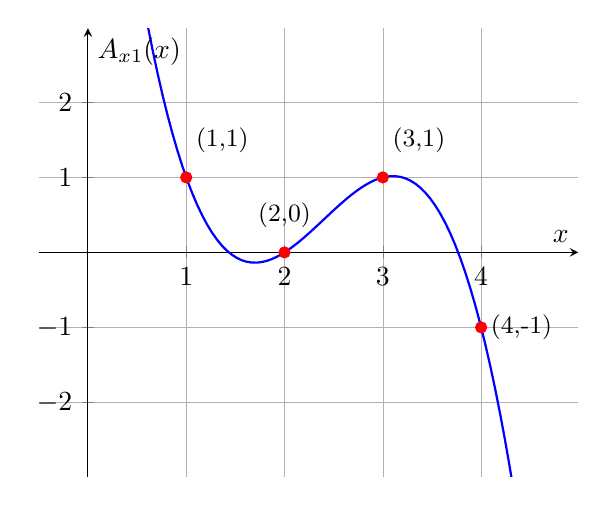
\begin{tikzpicture}
                \begin{axis}[
                    axis lines = middle,
                    xlabel = {$x$},
                    ylabel = {$A_{x1}(x)$},
                    ymin = -2.99, ymax = 2.99,
                    xmin = -0.5, xmax = 4.99,
                    domain = 0:5,
                    samples = 100,
                    ytick = {-3,...,3},
                    xtick = {0,1,...,5},
                    grid = both, 
                    grid style = {line width=.1pt, draw=gray!20},
                    major grid style = {line width=.2pt, draw=gray!60}
                ]
                \addplot[
                    color=blue,
                    thick
                ]
                {-5/6*x^3 + 6*x^2 - 79/6*x + 9};
                \addplot[
                    only marks,
                    mark=*,
                    color=red
                ]
                coordinates {(1,1) (2,0) (3,1) (4,-1)};
        
                \node at (axis cs:1,1.5) [anchor=west] {\small (1,1)};
                \node at (axis cs:2,0.2) [anchor=south] {\small (2,0)};
                \node at (axis cs:3,1.5) [anchor=west] {\small (3,1)};
                \node at (axis cs:4,-1) [anchor=west] {\small (4,-1)};
                
                \end{axis}
            \end{tikzpicture}
    
            \scriptsize\textbf{Illustration:} The Lagrange inteprolation polynomial for points $\{(1,1), (2,0), (3,1), (4,-1)\}$ visualized over $\mathbb{R}$.
        \end{center}
    \end{frame}

    \begin{frame}{Recap. QAP}
        \begin{figure}[H]
            \centering
            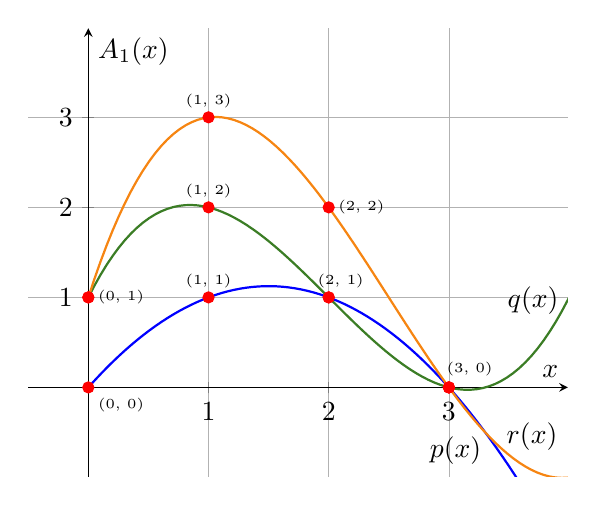
\begin{tikzpicture}
                \begin{axis}[
                    axis lines = middle,
                    xlabel = {$x$},
                    ylabel = {$A_1(x)$},
                    ymin = -0.99, ymax = 3.99,
                    xmin = -0.5, xmax = 3.99,
                    domain = 0:5,
                    samples = 100,
                    ytick = {-1,...,4},
                    xtick = {0,1,...,4},
                    grid = both,
                    grid style = {line width=.1pt, draw=gray!20},
                    major grid style = {line width=.2pt, draw=gray!60}
                ]

                % p(x)
                \addplot[
                    color=blue,
                    thick
                ]
                {3/2*x - 1/2*x^2};
                \addplot[
                    only marks,
                    mark=*,
                    color=red
                ]
                coordinates {(0, 0) (1, 1) (2, 1) (3, 0)};
                \node at (axis cs:3.35,-0.7) [anchor=east] {\text{$p(x)$}};

                \node at (axis cs:0,-0.2) [anchor=west] {\tiny (0, 0)};
                \node at (axis cs:1,1) [anchor=south] {\tiny (1, 1)};
                \node at (axis cs:2.1,1) [anchor=south] {\tiny (2, 1)};
                \node at (axis cs:2.9,0.2) [anchor=west] {\tiny (3, 0)};

                % q(x)
                \addplot[
                    color=OliveGreen,
                    thick
                ]
                {1/3*x^3 - 2*x^2 + 8/3*x + 1};
                \addplot[
                    only marks,
                    mark=*,
                    color=red
                ]
                coordinates {(0,1) (1,2) (2,1) (3, 0)};
                \node at (axis cs:3.7,0.7) [anchor=south] {\text{$q(x)$}};

                \node at (axis cs:0,1) [anchor=west] {\tiny (0, 1)};
                \node at (axis cs:1,2) [anchor=south] {\tiny (1, 2)};

                % r(x)
                \addplot[
                    color=BurntOrange,
                    thick
                ]
                {1/3*x^3 - 5/2*x^2 + 25/6*x + 1};
                \addplot[
                    only marks,
                    mark=*,
                    color=red
                ]
                coordinates {(0,1) (1,3) (2,2) (3, 0)};
                \node at (axis cs:3.4,-0.55) [anchor=west] {\text{$r(x)$}};

                \node at (axis cs:1,3) [anchor=south] {\tiny (1, 3)};
                \node at (axis cs:2,2) [anchor=west] {\tiny (2, 2)};

                \end{axis}
            \end{tikzpicture}
            \caption{Addition of two polynomials}
            \label{fig:example-polynomial-addition}
        \end{figure}
    \end{frame}

    \begin{frame}
        \vspace{-5pt}
        Now, using coefficients encoded with polynomials, we can build a constraint number 
        $X \in \{1, \dots\ m\}$ in the next way:
        \vspace{-5pt}
        \begin{align*}
            &(w_1A_1(X) + w_2A_2(X) + \dots + w_nA_n(X)) \times \\
            \times &(w_1B_1(X) + w_2B_2(X) + \dots + w_nB_n(X)) = \\ 
            = &(w_1C_1(X) + w_2C_2(X) + \dots + w_nC_n(X))
            \vspace{-5pt}
        \end{align*}
        \pause
        Or written more concisely:
        \vspace{-5pt}
        \begin{equation*}
            \left( \sum_{i = 1}^{n} w_iA_i(X) \right) \times \left( \sum_{i = 1}^{n} w_iB_i(X) \right) = \left( \sum_{i = 1}^{n} w_iC_i(X) \right)
        \end{equation*}   
        
        \vspace{-5pt}
        \begin{equation*}
            A(X) \times B(X) = C(X)
        \end{equation*}   
    \end{frame}

    \begin{frame}{Recap. QAP}
        Now, we can define a polynomial $M(X)$, that has zeros at all elements from the set
        $\Omega = \{1,\dots,m\}$
        \vspace{-5pt}
        \begin{equation*}
            M(X) = A(X) \times B(X) - C(X)
            \vspace{-5pt}
        \end{equation*}
        \pause
        It means, that $M(X)$ can be divided by \textbf{vanishing polynomial} $Z_{\Omega}(X)$ without a remainder!
        \vspace{-8pt}
        \begin{equation*}
            Z_{\Omega}(X) = \prod_{i=1}^m (X - i), \qquad \text{$H(X) = \frac{M(X)}{Z_{\Omega}(X)}$ is a polynomial}
            \vspace{-5pt}
        \end{equation*}
    \end{frame}

    \section{Encrypted Verification}

    \begin{frame}{Current Point}
        We've managed to encode into \textbf{a single polynomial} an entire computation (a program),
        of any size, independent of how much data it consumes. \\ \pause
        \vspace{10pt}
        Now, we need to figure our the protocol, how a prover can succinctly proof the knowledge of
        a correct witness for some circuit to a verifier, additionally, make it zero-knowledge and 
        non-interactive.\pause

        Where the knowledge of the correct witness is a knowledge of the quotient polynomial $H(X)$.
        \begin{equation*}
            M(X) = H(X) \times Z_{\Omega}(X)
        \end{equation*}
    \end{frame}

    \begin{frame}{Notation Preliminaries}
        In this section we'll use a group of points on elliptic curve denoted as $\mathbb{G}$ of
        prime order $q$ with a generator $g$.\\ \pause
        \vspace{5pt}
        The symmetric pairing function $e: \mathbb{G} \times \mathbb{G} \to \mathbb{G}_T$, where
        $(\mathbb{G}_T, \times)$ is a target group.
    \end{frame}

    \begin{frame}{Naive Proof}
        Suppose, we are given a circuit $\mathcal{C}$ with a maximum degree $d$ of polynomials
        used underneath.
        
        Thus, all parties additionally know the target polynomial $Z(x)$ and QAP polynomials 
        $\{L_i(x)\}_{i \in [n]}, \{R_i(x)\}_{i \in [n]}, \{O_i(x)\}_{i \in [n]}$, where $n$ is 
        number of witness elements.

        \pause
        \textbf{Prover}
        \vspace{-5pt}
        \begin{itemize}[label=\ding{51}]
            \item \vspace{-3pt} Provides witness $\boldsymbol{w}$ to a Verifier.
        \end{itemize}
        \pause
        \textbf{Verifier}
        \vspace{-5pt}
        \begin{itemize}[label=\ding{51}]
            \item \vspace{-3pt} Checks $\left( \sum_{i = 1}^{n} w_iA_i(X) \right) \times \left( \sum_{i = 1}^{n} w_iB_i(X) \right) = \left( \sum_{i = 1}^{n} w_iC_i(X) \right)$
        \end{itemize}
    \end{frame}

    \begin{frame}{Naive Proof}
        \begin{itemize}
            \item[\ding{55}] Succint
            \item[\ding{51}] Non-Interactive
            \item[\ding{55}] Zero-Knowledge
        \end{itemize}

        \pause
        \vspace{20pt}
        \begin{columns}
            \begin{column}{0.7\textwidth}
                The verifier could actually just run a program that represents a circuit 
                $\mathcal{C}$ on witness data $\boldsymbol{w}$.
            \end{column}

            \begin{column}{0.2\textwidth}
                
\includegraphics[width=\linewidth]{../presentations/images/common/new-moon-with-face.jpg}
            \end{column}
        \end{columns}\pause

        We, definitely, need to encrypt the witness data $\boldsymbol{w}$ somehow...
    \end{frame}

    \begin{frame}
        Let's define the \textit{encryption} operation as follows:
        \vspace{-10pt}
        \begin{equation*}
            \mathsf{Enc}: \mathbb{F} \to \mathbb{G}, \quad \mathsf{Enc}(x) := g^x
            \vspace{-5pt}
        \end{equation*}\pause
        Essentially, $\mathsf{Enc}(p(\tau))$ is the \textbf{KZG Commitment}. 
        \begin{example}
            Consider the polynomial: $p(x) = x^2 - 5x + 2$, the encryption of $p(\tau)$:
            {\large
            \begin{equation*}
                \mathsf{Enc}(p(\tau)) = g^{p(\tau)} = g^{\left( \tau^2 - 5\tau + 2 \right)}  = \left( g^{\tau^2} \right)^1 \cdot {\left( g^{\tau^1} \right)}^{-5} \cdot \left(g^{\tau^0}\right)^2
            \end{equation*}}
        \end{example}\pause
        \begin{alertblock}{Question}
            KZG Commitment requires encrypted powers of $\tau$: $\{g^{\tau^i}\}_{i \in [d]}$. But 
            where the prover can take them?
        \end{alertblock}
    \end{frame}

    \begin{frame}{Trusted Setup}
        \textbf{Trusted Party Setup}
        \vspace{-5pt}
        \begin{itemize}[label=\ding{51}]
            \item \vspace{-3pt} Picks a random value $\tau \xleftarrow{R} \mathbb{F}$. \pause
            \item \vspace{-3pt} Calculates the public parameters $\{g^{\tau^i}\}_{i \in [d]}$.\pause
            \item \vspace{-3pt} \textbf{Deletes} $\tau$ (toxic waste).\pause
            \item \vspace{-3pt} \textbf{Outputs} prover parameters $\mathsf{pp} \gets \{g^{\tau^i}\}_{i \in [d]}$ and verifier parameters $\mathsf{vp} \gets \mathsf{com}(Z)$. \pause
        \end{itemize} \pause

        This way, we can find the KZG commitment for each polynomial. For example:
        \begin{equation*}
            \mathsf{com}(L) \triangleq g^{L(\tau)} = g^{\sum_{i=0}^d L_i \tau^i} = \prod_{i=0}^d (g^{\tau^i})^{L_i},
        \end{equation*}
    \end{frame}

    \begin{frame}
        Now, we can calculate:
        \begin{equation*}
            g^{L(\tau)}, g^{R(\tau)}, g^{O(\tau)}, g^{H(\tau)}, g^{Z(\tau)}
        \end{equation*}
        But how can we verify $H(x)Z(x) = L(x)R(x) - O(x)$ in the ecnrypted space? 
        
        Well, first notice that the check is equivalent to:
        \begin{equation*}
            L(\tau)R(\tau) = Z(\tau)H(\tau) + O(\tau).
        \end{equation*}
        So, we can check this equality as follows:
        \begin{equation*}
            e(\mathsf{com}(L), \mathsf{com}(R)) = e(\mathsf{com}(Z), \mathsf{com}(H)) \cdot e(\mathsf{com}(O), g),
        \end{equation*}
    \end{frame}

    \begin{frame}
        \scriptsize

        \textbf{Trusted Setup: }
        $\tau \xleftarrow{R} \mathbb{F} \textbf{,} \quad \{g^{\tau^i}\}_{i \in [d]}\textbf{,} \quad$ \textbf{delete}($\tau$).
        \vspace{10pt}

        \tikzset{
            arrow/.style={-latex, ultra thick}
        }

        \begin{center}
            \begin{tikzpicture}
                \node[inner sep=0pt, align=center] (prover) at (-3.5, -3) {
                    
\includegraphics[width=2cm]{images/common/prover.png}\\Prover $\mathcal{P}$
                };

                \node[inner sep=0pt, align=center] (verifier) at (4, -3) {
                    
\includegraphics[width=2cm]{images/common/verifier.png}\\Verifier $\mathcal{V}$
                };
                
                \onslide<2->{
                    \node[inner sep=0pt, align=center] (pdata) at (-3, -0.6) {
                        \begin{minipage}{4cm}
                            \begin{itemize}[label=\ding{51}]
                                \item $H(x) = \frac{L(x) \times R(x) - O(x)}{Z(x)}$.
                                \onslide<3->{\item {
                                    KZG commitments: 
                                    \vspace{-10pt}
                                    \begin{align*}
                                        \pi_L &\gets \mathsf{com}(L), &\pi_R &\gets \mathsf{com}(R), \\ 
                                        \pi_O &\gets \mathsf{com}(O), &\pi_H &\gets \mathsf{com}(H),
                                    \end{align*}
                                }}
                            \end{itemize}
                        \end{minipage}
                    };
                }

                \onslide<4->{
                    \draw[arrow] (prover) -- (verifier) node[midway, above=1mm] {$\boldsymbol{\pi} = (\pi_L,\pi_R,\pi_O,\pi_H)$};
                }

                \onslide<5->{
                    \node[inner sep=0pt, align=center] (vdata) at (5, -1.1) {
                        \begin{minipage}{6cm}
                            \begin{itemize}[label=\ding{51}]
                                \item $e(\pi_L, \pi_R) == \\ e(\mathsf{com}(Z), \pi_H) \cdot e(\pi_O, g)$.
                            \end{itemize}
                        \end{minipage}
                    };
                }
            \end{tikzpicture}
        \end{center}
    \end{frame}

    \begin{frame}
        \begin{itemize}
            \item[\ding{51}] Succint
            \item[\ding{51}] Non-Interactive
            \item[\ding{51}] Zero-Knowledge \pause
            \item[\ding{55}] \vspace{7pt} Does it work?
        \end{itemize}
    \end{frame}

    \begin{frame}{Why it doesn't work??}\begin{adjustwidth}{-5mm}{0mm}
        \scriptsize

        \textbf{Trusted Setup: }
        $\tau \xleftarrow{R} \mathbb{F} \textbf{,} \quad \{g^{\tau^i}\}_{i \in [d]}\textbf{,} \quad$ \textbf{delete}($\tau$).
        \vspace{10pt}

        \tikzset{
            arrow/.style={-latex, ultra thick}
        }

        \begin{center}
            \begin{tikzpicture}
                \node[inner sep=0pt, align=center] (prover) at (-3.5, -2.4) {
                    
\includegraphics[width=2cm]{images/common/prover.png}\\Prover $\mathcal{P}$
                };

                \node[inner sep=0pt, align=center] (verifier) at (4, -2.4) {
                    
\includegraphics[width=2cm]{images/common/verifier.png}\\Verifier $\mathcal{V}$
                };
                
                \onslide<2->{\node[inner sep=0pt, align=center] (pdata) at (-2.3, 0) {
                    \begin{minipage}{6cm}
                        \begin{itemize}[label=\ding{51}]
                            \onslide<3->{\item $H^{\prime}(x) \xleftarrow{R} \mathbb{F}[x], \quad M^{\prime}(x) = Z(x) \times H^{\prime}(x)$.}
                            \onslide<4->{\item Finds $L^{\prime}(x), R^{\prime}(x), O^{\prime}(x)$ such that: \\ $L^{\prime}(x) \times R^{\prime}(x) - O^{\prime}(x) = M^{\prime}(x)(x)$}
                            \onslide<5->{\item {
                                KZG commitments: 
                                \vspace{-10pt}
                                \begin{align*}
                                    \pi_{L^{\prime}(x)} &\gets \mathsf{com}(L^{\prime}(x)), &\pi_{R^{\prime}(x)} &\gets \mathsf{com}(R^{\prime}(x)), \\ 
                                    \pi_{O^{\prime}(x)} &\gets \mathsf{com}(O^{\prime}(x)), &\pi_{H^{\prime}(x)} &\gets \mathsf{com}(H^{\prime}(x)),
                                \end{align*}
                            }}
                        \end{itemize}
                    \end{minipage}
                };}

                \onslide<6->{\draw[arrow] (prover) -- (verifier) node[midway, above=1mm] {$\boldsymbol{\pi} = (\pi_{L^{\prime}(x)},\pi_{R^{\prime}(x)},\pi_{O^{\prime}(x)},\pi_{H^{\prime}(x)})$};}

                \onslide<7->{\node[inner sep=0pt, align=center] (vdata) at (5.1, -0.6) {
                    \begin{minipage}{6cm}
                        \begin{itemize}[label=\ding{51}]
                            \item $e(\pi_{L^{\prime}(x)}, \pi_{R^{\prime}(x)}) == \\ e(\mathsf{com}(Z), \pi_H) \cdot e(\pi_{O^{\prime}(x)}, g)$.
                        \end{itemize}
                    \end{minipage}
                };}
            \end{tikzpicture}
        \end{center}

        \pause
        \begin{block}{Problem}
            Prover isn't forced to use the values from the trusted setup.
        \end{block}
    \end{adjustwidth}\end{frame}

    \begin{frame}{Proof Of Exponent}
        \scriptsize

        \textbf{Trusted Setup: }
        $\tau, \textcolor{green!50!black}{\alpha} \xleftarrow{R} \mathbb{F} \textbf{,} \quad \{ \{g^{\tau^i}\}_{i \in [d]}\textbf{,} \quad \textcolor{green!50!black}{\{g^{\alpha \tau^i}\}_{i \in [d]}} \} \textbf{,} \quad$ \textbf{delete}($\tau, \textcolor{green!50!black}{\alpha}$).
        \vspace{10pt}

        \tikzset{
            arrow/.style={-latex, ultra thick}
        }

        \begin{center}
            \begin{tikzpicture}
                \node[inner sep=0pt, align=center] (prover) at (-3.5, -3) {
                    
\includegraphics[width=2cm]{images/common/prover.png}\\Prover $\mathcal{P}$
                };

                \node[inner sep=0pt, align=center] (verifier) at (4, -3) {
                    
\includegraphics[width=2cm]{images/common/verifier.png}\\Verifier $\mathcal{V}$
                };
                
                \onslide<2->{\node[inner sep=0pt, align=center] (pdata) at (-3, -0.6) {
                    \begin{minipage}{4cm}
                        {\tiny\begin{itemize}[label=\ding{51}]
                            \item $H(x) = \frac{L(x) \times R(x) - O(x)}{Z(x)}$.
                            \onslide<3->{\item {
                                KZG commitments: 
                                \vspace{-8pt}
                                \begin{align*}
                                    \pi_L &\gets g^{L(\tau)}, \quad &\pi_L' &\gets g^{\alpha L(\tau)},\\[-2pt]
                                    \pi_R &\gets g^{R(\tau)}, \quad &\pi_R' &\gets g^{\alpha R(\tau)},\\[-2pt]
                                    \pi_O &\gets g^{O(\tau)}, \quad &\pi_O' &\gets g^{\alpha O(\tau)},\\[-2pt]
                                    \pi_H &\gets g^{H(\tau)}, \quad &\pi_H' &\gets g^{\alpha H(\tau)}.
                                \end{align*}
                            }}
                        \end{itemize}}
                    \end{minipage}
                };}
            
                \onslide<4->{\draw[arrow] (prover) -- (verifier) node[midway, above=1mm] {$\boldsymbol{\pi} = (\pi_L,\pi_R,\pi_O,\pi_H)$};}

                \onslide<5->{\node[inner sep=0pt, align=center] (vdata) at (5, -0.6) {
                    \begin{minipage}{4cm}
                        {\tiny\begin{itemize}[label=\ding{51}]
                            \item $e(\pi_L, \pi_R) ==\\ e(\mathsf{com}(Z), \pi_H) \cdot e(\pi_O, g)$.
                            \onslide<6->{\item {
                                Proof of Exponent:
                                \vspace{-8pt}
                                \begin{align*}
                                    e(\pi_L, g^{\alpha}) &= e(\pi_L', g), \qquad\qquad\qquad\\[-2pt] %quads are to adjust spacing on the slide
                                    e(\pi_R, g^{\alpha}) &= e(\pi_R', g), \\[-2pt]
                                    e(\pi_O, g^{\alpha}) &= e(\pi_O', g), \\[-2pt]
                                    e(\pi_H, g^{\alpha}) &= e(\pi_H', g).
                                \end{align*}
                            }}
                        \end{itemize}}
                    \end{minipage}
                };}
            \end{tikzpicture}
        \end{center}
    \end{frame}

    \begin{frame}{Including PoE}
        \begin{itemize}
            \item[\ding{51}] Succint
            \item[\ding{51}] Non-Interactive
            \item[\ding{51}] Zero-Knowledge \pause
            \item[\ding{55}] Sound
        \end{itemize}

        \pause
        \vspace{15pt}
        \begin{block}{Problem}
            There is no guarantee that the same witness $\mathbf{w}$ was used to calculate all the commitments $\pi_L, \pi_R, \pi_O, \pi_H$.
        \end{block}
    \end{frame}

    \section{Make It Sound}

    \begin{frame}{Additional Optimization}
        Recal that:
        \begin{equation*}
            L(x) = \sum_{i=0}^n w_iL_i(x), \quad R(x) = \sum_{i=0}^n w_i R_i(x), \quad O(x) = \sum_{i=0}^n w_iO_i(x).
        \end{equation*}

        \pause

        Here public data is:
        \begin{equation*}
            \{L_i(x)\}_{i \in [n]}, \{R_i(x)\}_{i \in [n]}, \{O_i(x)\}_{i \in [n]}
        \end{equation*}

        \pause
        
        Moreover, it's defined only by the circuit and trusted setup, thus, it can calculated before proof generation as a part of the trusted setup.
    \end{frame}

    \begin{frame}{Additional Optimization}
        Updated Trusted Setup:
        \vspace{-10pt}
        {\scriptsize \begin{align*}
            \{g^{\tau^i}\}_{i \in [d]}&, \quad \{g^{\alpha \tau^i}\}_{i \in [d]}, \\
            \textcolor{green!50!black}{\{g^{L_i(\tau)}\}_{i \in [n]}}&, \quad \textcolor{green!50!black}{\{g^{\alpha L_i(\tau)}\}_{i \in [n]}},\\ 
            \textcolor{green!50!black}{\{g^{R_i(\tau)}\}_{i \in [n]}}&, \quad \textcolor{green!50!black}{\{g^{\alpha R_i(\tau)}\}_{i \in [n]}},\\
            \textcolor{green!50!black}{\{g^{O_i(\tau)}\}_{i \in [n]}}&, \quad \textcolor{green!50!black}{\{g^{\alpha O_i(\tau)}\}_{i \in [n]}}  
        \end{align*}}
       
        \pause
        
        Consider the polynomial $L(x) = \sum_{i=0}^n w_iL_i(x)$. 
        
        \pause
        
        $\mathcal{P}$ can compute the KZG commitment $\pi_L$ and its PoE $\pi_L'$ as follows:
        \begin{align*}
            \pi_L &\triangleq g^{L(\tau)} = g^{\sum_{i=0}^n w_i L_i(\tau)} = \prod_{i=0}^n (g^{L_i(\tau)})^{w_i}, \\
            \pi_L' &\triangleq g^{\alpha L(\tau)} = g^{\alpha \sum_{i=0}^n w_i L_i(\tau)} = \prod_{i=0}^n (g^{\alpha L_i(\tau)})^{w_i}.
        \end{align*}
    \end{frame}

    \begin{frame}{Witness Consistency Check}
        \begin{block}{Problem}
            Prover isn't forced to use the same witness while calculating commitments.
        \end{block}
        
        To prove that the same $\mathbf{w}$ is used in all commitments, we need some ``checksum''
        term that will somehow combine all polynomials $L(x)$, $R(x)$, and $O(x)$ with the witness
        $\mathbf{w}$.

        \pause
        Hmm... Let's introduce one more coefficient:
        \begin{equation*}
            \beta \xleftarrow{R} \mathbb{F}.
        \end{equation*}
    \end{frame}

    \begin{frame}[plain, standout]
        \centering
        \LARGE
        \textbf{Thank you for your attention} \\
        
        \vspace{0.2cm} \Huge \ding{170} \large \\
        
        \vspace{1cm}
  
        \href{https://zkdl-camp.github.io/}{\raisebox{-.1em}{\hspace{.025em}\faIcon{globe}}\hspace{.325em}zkdl-camp.github.io} \\
  
        \href{https://github.com/ZKDL-Camp}{\raisebox{-.1em}{\hspace{.025em}\faIcon{github}}\hspace{.325em}github.com/ZKDL-Camp}
        
        \begin{center}
            
\includegraphics[width=0.15\textwidth]{images/logo.png}
        \end{center}
    \end{frame}
\end{document}